\documentclass[11pt]{article}
\usepackage[utf8]{inputenc}
\usepackage{amsmath}
\usepackage{amsfonts}
\usepackage{amssymb}
\usepackage{graphicx}
\usepackage[hidelinks, colorlinks=True, urlcolor=blue, linkcolor=black]{hyperref}
\usepackage[a4paper, margin=1in]{geometry}
\usepackage{math}
% \usepackage{newtx}
\usepackage{dsfont}
\usepackage{setspace}
\usepackage{titlesec}
\titleformat*{\section}{\large\bfseries}
\titleformat*{\subsection}{\normalsize\bfseries}
\titleformat*{\subsubsection}{\normalsize\itshape}

\linespread{1.1}

\title{
    Monetary and Fiscal Policy Regime Changes\footnote{Code available at \href{https://github.com/sidd3888/HAMacroCompEx}{\texttt{https://github.com/sidd3888/HAMacroCompEx}}}\\
    \Large ECON-33540: Macroeconomics with Heterogeneous Households
}
\author{Siddarth Venkatesh}
\date{March 23, 2026}

\begin{document}

\maketitle

% \onehalfspacing

\section{Introduction}

In this project, I analyze the effects of changes in the monetary and fiscal policy rules on the transition path of the economy in response to a shock. I illustrate these effects using two different shocks, a positive TFP shock and a positive discount rate shock. I also study how knowledge of the impending regime change affects the transition path of the economy. I find that unforeseen regime changes can lead to jumps in control variables that might not necessarily move them toward the transition path under the second regime alone. Additionally, I find that advance knowledge of an impending regime change can lead to a transition path that is dissimilar to the transition path under either regime alone, and might not represent a ``middle ground'' between the two.

\section{Model}

\subsection{Consumers}

I will build on the textbook HANK model developed in class, with a unit mass of consumers solving the problem described by the HJB:
\begin{align*}
    \rho V(a,\,z,\,t) &= \max_{c,\,h} E_t\,\, u(c) - v(h) + \partial_{a}V(a,\,z,\,t)\cdot \bp{r(t)a + w(t)zh + z\Pi(t) - \tau(z,\,t) - c} \\&+ \sum_{z' \in \mathcal{Z}} \l_{z,\,z'} \cdot (V(a,\,z',\,t) - V(a,\,z,\,t)) + \partial_{t}V(a,\,z,\,t)\\
    \text{s.t.} \dot{a} &= r(t)a + w(t)zh + z\Pi(t) - \tau(z,\,t) - c
\end{align*}
where $z$ is an idiosyncratic productivity process with mean under the stationary distribution equal to 1, $a$ is the level of the consumer's assets, $c$ is consumption, $h \in \bs{0,\,\bar{h}}$ is hours worked, $\Pi(t)$ is the total dividend paid by firms, and $\tau(z,\,t)$ is the tax net transfers paid by the consumer of type $z$ at time $t$. The functions $u$ and $v$ are of the form:
\begin{align*}
    u(c) &= \frac{c^{1-\sigma}}{1 - \sigma} \\
    v(h) &= \psi \cdot \frac{h^{1+\gamma}}{1 + \gamma}
\end{align*}
where $\sigma$ is the coefficient of relative risk aversion and $1/\gamma$ is the Frisch elasticity of labor supply. The tax schedule $\tau$ is of the form:
\begin{align}
    \tau(z,\,t) &= \bs{\tau_1z - \tau_0(t)}Y^*
\end{align}
where $Y^*$ is steady state output. The only difference so far in the model described here and the model in class is the expectations operator in the HJB, which allows for the possibility of regime changes in monetary and fiscal policy that are unknown to agents. I will focus on one of two possibilities. Either consumers have perfect foresight about an impending regime change, or they incorrectly assume that there will be no regime change when in fact there will be one.

\subsection{Firms}

The final good firm is competitive, and produces the consumption good using CES technology, solving the static problem:
\begin{align*}
    \max_{Y(i)} \bp{\int_{0}^{1}Y(i)^{\frac{\epsilon - 1}{\epsilon}}di}^{\frac{\epsilon}{\epsilon - 1}} - \int_{0}^{1}\frac{p(i)}{P}Y(i)di
\end{align*}
where $p(i)$ is the price of good $i$ and $P$ is the price of the final good. The solution to this problem yields the demand for good $i$:
\begin{align*}
    Y(i) &= \bp{\frac{p(i)}{P}}^{-\epsilon}Y
\end{align*}
The intermediate good firms are monopolistically competitive and maximize expected present value of lifetime profits, taking the demand function as given. Their profits, $\Pi(i,\,t)$, in each period are:
\begin{align*}
    \Pi(i, t) = p(i,\,t)Y(i,\,t) - w(t)L(i,\,t) - \underbrace{\frac{\theta}{2}\bp{\frac{\dot{p}(i,\,t)}{p(i,\,t)} - \pi^*}^2Y(t)}_{\equiv \Theta(t)}
\end{align*}
such that $Y(i,\,t) = A(t)L(i,\,t)$ and $\pi^*$ is the inflation target of the central bank. $A(t)$ is total factor productivity and $\Theta(t)$ is the cost of price adjustment. Since all intermediate good firms are identical, $p(i,\,t) = P(t)$ and $Y(i,\,t) = Y(t)$. The path of inflation is described by the Phillips curve:
\begin{align*}
    \bp{r(t) - \frac{\dot{Y}(t)}{Y(t)}}(\pi(t) - \pi^*) &= \frac{\e}{\t}\bp{\frac{w(t)}{A(t)} - \frac{\e - 1}{\e}} + \dot{\pi}(t)
\end{align*}
except at the time of the regime change in an imperfect foresight equilibrium, where there can be a jump in the inflation rate.

I assume that firms have perfect foresight about the regime change if and only if consumers do, considering that firms are owned by consumers, but also in part due to it simplifying the solution.

\subsection{Monetary and Fiscal Policy}

The government issues short term debt, with the level of real government debt at time $t$ denoted by $B(t)$. The evolution of government debt is described by:
\begin{align*}
    \dot{B}(t) &= r(t)B(t) - s(t)
\end{align*}
where $s(t) = (\tau_1 - \tau_0(t))Y^*$ is the government's primary surplus. The government adjusts its surplus according to the following feedback rule:
\begin{align*}
    s(t) &= s^* + \phi_b(t)(B(t) - B^*) + \vartheta(t)
\end{align*}
where $s^*$ is the steady state primary surplus, $B^*$ is the steady state level of government debt, $\phi_b(t)$ is the time dependent surplus adjustment parameter, and $\vartheta(t)$ is a fiscal shock. The central bank, meanwhile, sets the nominal interest rate according to:
\begin{align*}
    i(t) &= i^* + \phi_{\pi}(t)(\pi(t) - \pi^*) + \varepsilon(t)
\end{align*}
where $i^*$ is the steady state nominal interest rate, $\pi(t)$ is the inflation rate at time $t$, $\phi_{\pi}(t)$ is the time dependent inflation feedback parameter, and $\varepsilon(t)$ is a monetary shock. The regime change that I will focus on in this project, which will restrict the form of $\phi_b(t)$ and $\phi_{\pi}(t)$, is a change of the following form:
\begin{align*}
    \phi_b(t) &= \begin{cases}
        \phi_b^1 & t < T_0 \\
        \phi_b^2 & t \geq T_0
    \end{cases} \\
    \phi_{\pi}(t) &= \begin{cases}
        \phi_{\pi}^1 & t < T_0 \\
        \phi_{\pi}^2 & t \geq T_0
    \end{cases}
\end{align*}
where $T_0$ is the time of the regime change. Let $T_0 = \infty$ denote the case where there is no regime change.

\subsection{Equilibrium}

Given the two types of information scenarios described above, there are naturally two types of equilibria to consider. The first is a perfect foresight equilibrium, where agents know that there is a regime change at time $T_0$ if $T_0 < \infty$, and the equilibrium satisfies all the criteria of a standard recursive competitive equilibrium in the HANK model from class, except for the fact that given a path of real rates (which need not be continuous), the nominal interest rate and inflation satisfy the time dependent monetary policy rule, and government debt and lump-sum transfers, $\tau_0(t)$, follow the time dependent fiscal policy rule. In this equilibrium, since consumers receive information of the shock and the impending regime change together, the smoothing motive will ensure that consumption and hours worked will follow a continuous path. Since the monopolistic firms also solve a perfect foresight problem, the inflation rate will also follow a continuous path, and output will also be continuous in time.

The second type of equilibrium is an imperfect foresight equilibrium. Here, agents are fully aware of any shock and its dissipation at the time it hits, but do not know that the monetary and fiscal authorities plan a regime change at time $T_0 < \infty$ even if there is one. This equilibrium can also be defined using the standard recursive competitive equilibrium. Precisely, the equilibrium is characterized till time $T_0$ by a perfect foresight equilibrium with $T_0 = \infty$ and the initial monetary and fiscal policy rules. From time $T_0$, it is equivalent to a perfect foresight equilibrium with $T_0 = \infty$ and the new monetary and fiscal policy rules, but with initial conditions on the distribution over assets and income states given by the distribution at time $T_0$ under the first perfect foresight equilibrium. In this equilibrium, since consumers and firms receive new information at time $T_0$, we expect to see control variables jump at $T_0$.

\subsection{Computation}

The logic of the computation closely follows the manner in which the two types of equilibria were defined.\footnote{While the algorithm is mine, I acknowledge the aid of LLMs in implementing it.} For the perfect foresight equilibrium, note that the consumer problem is still solved by backward iteration of the HJB, with the evolution of the distribution governed by the corresponding KFE that can be solved using forward iteration. The only difference is that given a guess for the path of inflation and output, the path of interest rates and government debt, surplus, and therefore lump-sum transfers to the consumers are now determined by time varying monetary and fiscal policy rules. When solving for government debt, I use the direction of iteration implied by the feedback rule after the regime change (though in the analysis that follows, all parameterizations imply backward iteration).

For the imperfect foresight equilibrium, the computation is split into two pieces. Since the monetary and fiscal policy rules are instantaneous and only take into account the current level of inflation and government debt, the equilibrium path before the regime change is the same as the one in the absence of a regime change. Hence, I solve for the transition path for the standard model without a regime change, which yields a sequence of aggregate variables and distributions. Then, solving for the second segment also involves using the same algorithm to solve for transition paths, but with the initial condition being determined by the distribution at time $T_0$ rather than the stationary distribution. Then, like previously, we can compute the second half of the equilibrium path using the new monetary and fiscal policy rules. The algorithm allows for the possibility of a jump in control variables at $T_0$, thus requiring two guess values for inflation at $T_0$. As a result, we can implement an additional market clearing condition requiring the government debt calculated from the first half of the equilibrium path to be equal to the government debt calculated from the second half of the equilibrium path at $T_0$.

\subsubsection*{Limitation}

The one case where this algorithm does not converge is when the shock is a fiscal stimulus shock. Particularly, when the regime change is from passive money - active fiscal to active money - passive fiscal, the algorithm fails to converge for the imperfect foresight equilibrium. On the other hand, it fails to converge for a change from active money - passive fiscal to passive money - active fiscal for the perfect foresight equilibrium. My conjecture is that this is due to the construction of the government debt sequence. Nevertheless, I omit an analysis of regime change on fiscal stimulus shocks due to this reason.

\subsection{Parameterization}

I use the same parameterization of the model as in the slides, with the following changes. The decay rate of shocks is set to 0.2, and $T_0$ is set to 8 quarters after the initial shock. This is so that the regime change occurs not too soon after the initial shock, but the shock has not entirely dissipated. Even with such a small portion of the initial shock still undissipated (20 percent), the effect of an unforeseen regime change can be seen to be significant. I also instantiate a time grid that is finer around $T_0$ to better capture transition dynamics around the regime change. The two regimes I test are as follows:
\begin{align*}
    \text{Regime 1:} &\quad \phi_b = 0.0,\,\, \phi_{\pi} = 0.0 \\
    \text{Regime 2:} &\quad \phi_b = 0.1,\,\, \phi_{\pi} = 1.1
\end{align*}
I test the effect of a change from regime 1 to regime 2, which is a change from passive money - active fiscal to active money - passive fiscal, in response to two different shocks to compare transition dynamics and the effect of foresight about the regime change.

\section{Results}

\subsection{Positive TFP shock}

\subsubsection*{Baseline: No regime change}

We consider the transition path of the economy under Regime 1 alone, as in Figure \ref{fig:tfp}, as the baseline from which we depart.
\begin{figure}[h]
    \centering
    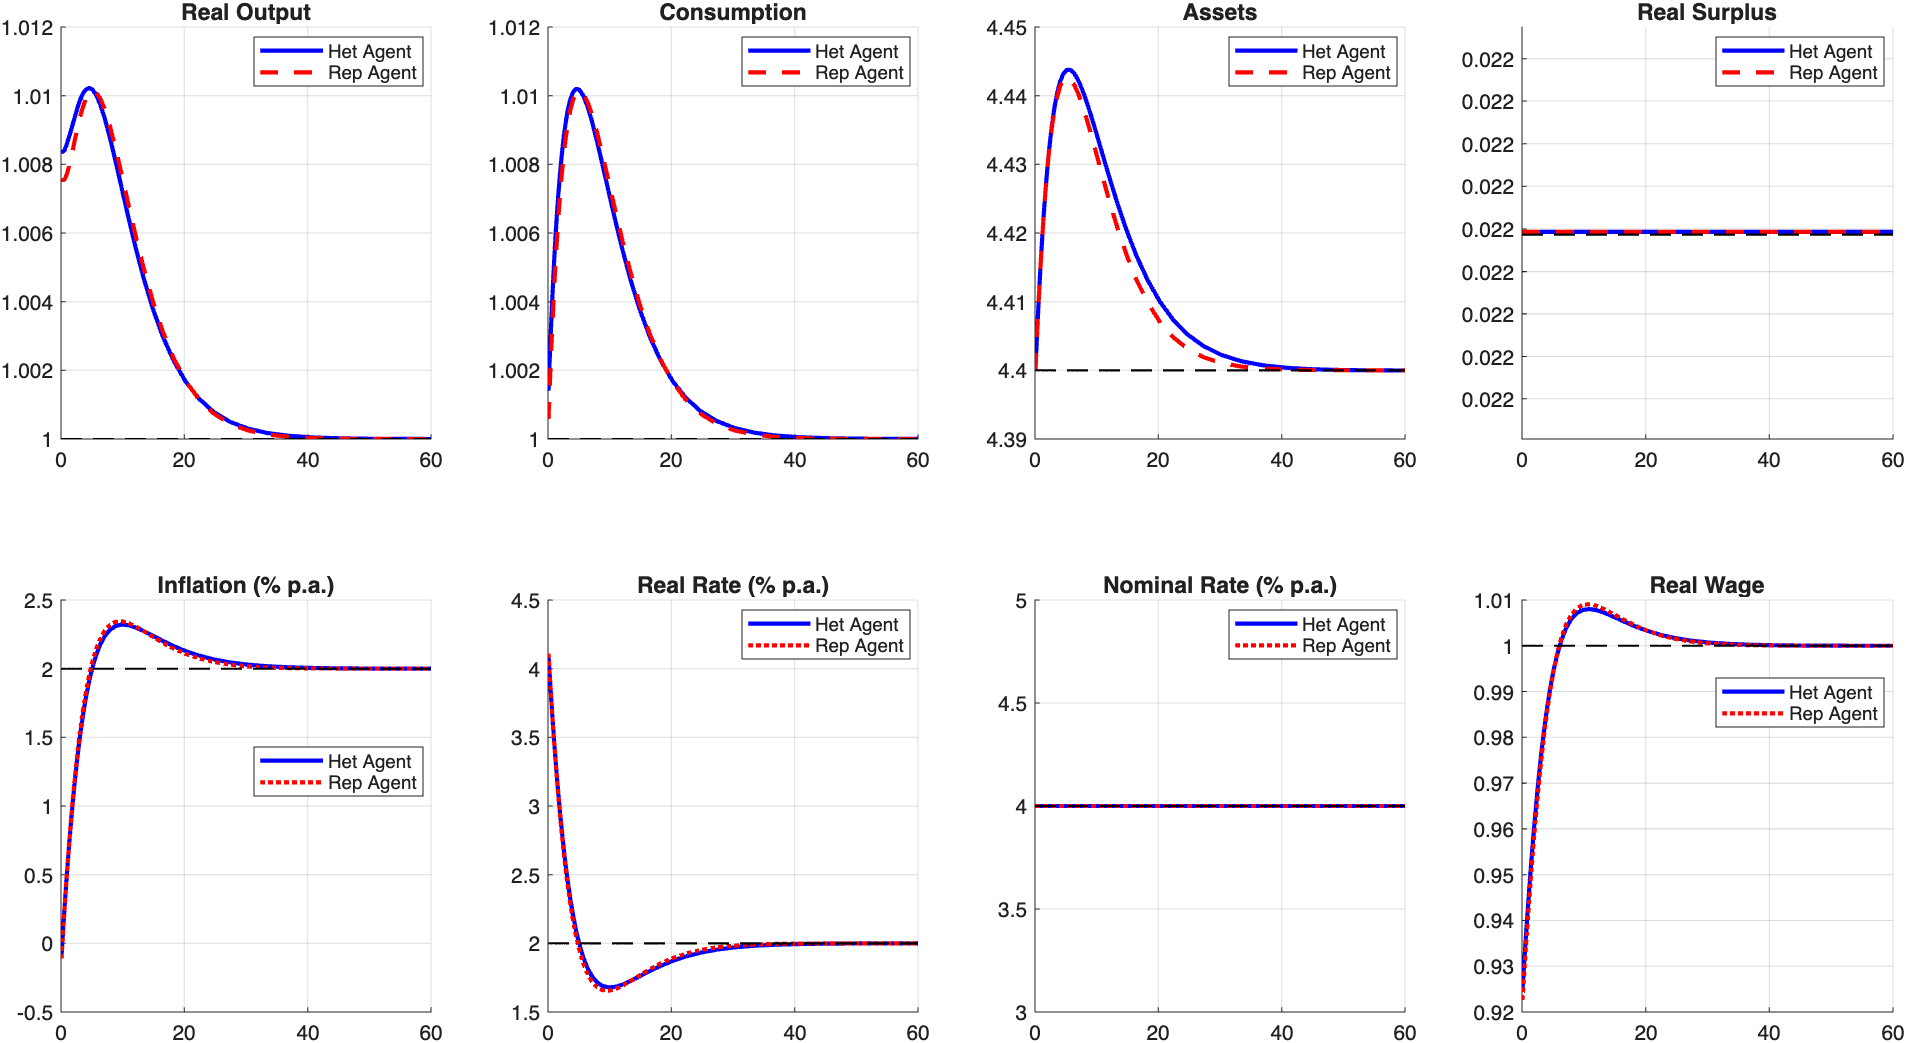
\includegraphics[width=0.8\textwidth]{Figures/TFP_HARA_reg1.png}
    \caption{Transition path after a 5\% TFP shock: Regime 1}
    \label{fig:tfp}
\end{figure}
A positive TFP shock leads to an initial decrease in marginal costs and real wages, leading to an increase in real output and a decrease in inflation. The decrease in real wages results in a decrease in hours worked, hence increasing output by less than 1\%. With the nominal rate pegged at $i^*$, the real rate increases with a fall in inflation, which means the increase in consumption is further dampened by an increased incentive to save. This leads to a steady accumulation of assets. As the real rate falls and real wages rise, hours worked and output increase for a short period, along with an increase in inflation above the target. As the TFP shock continues to dissipate and real wages exceed the steady state level, output starts to fall, and agents start to dissave. Inflation remains above the target for over 30 quarters, as the economy eventually returns to the steady state.

\subsubsection*{Imperfect foresight equilibrium}

The transition path of the economy in response to a TFP shock under an imperfect foresight equilibrium is seen in Figure \ref{fig:tfp_unknown}.
\begin{figure}[h]
    \centering
    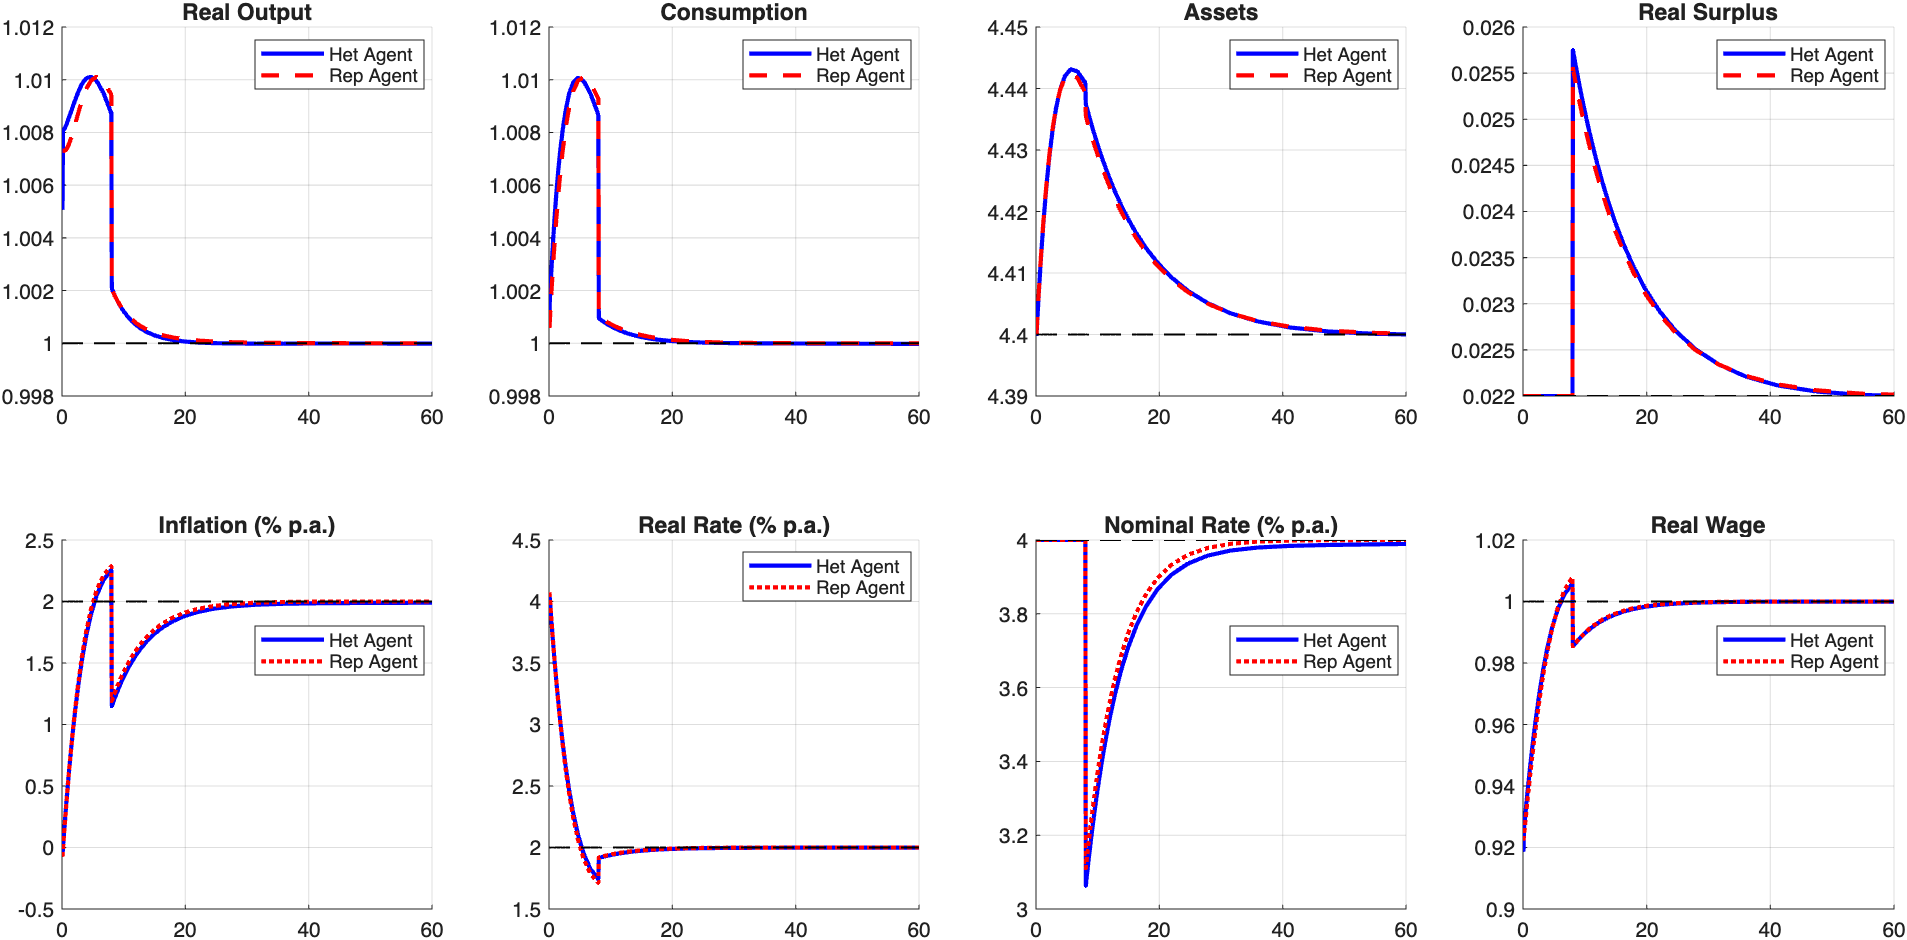
\includegraphics[width=0.8\textwidth]{Figures/TFP_unknown_1_HARA.png}
    \caption{Imperfect foresight equilibrium after a 5\% TFP shock}
    \label{fig:tfp_unknown}
\end{figure}
The transition path for the first 8 quarters, i.e. until $T_0$, is identical in the imperfect foresight equilibrium as in the baseline. However, at $T_0$, agents learn of the regime changes in monetary and fiscal policy. Primarily, they learn that the government will now maintain surpluses above steady state level to quickly repay the increased debt they accumulated over the initial period of asset accumulation. Agents are now taxed more, and their disposable incomes fall, leading to a decrease in consumption and the start of the dissaving phase due to the smoothing motive.

In the absence of a change in wage, an increase in the marginal utility of consumption implies an increased incentive to work, which results in a fall in the real wage to bring the labor market back to equilibrium. Real output falls, and so does inflation, which falls below the target. In response, the central bank cuts the nominal interest rate, which keeps the real rate below the steady state level. Over time, as the shock fully dissipates and government debt and household assets return to steady state, all other variables return to their steady state levels as well.

\subsubsection*{Perfect foresight equilibrium}

Advance knowledge of the regime change invokes a vastly different response to the TFP shock.
\begin{figure}[h]
    \centering
    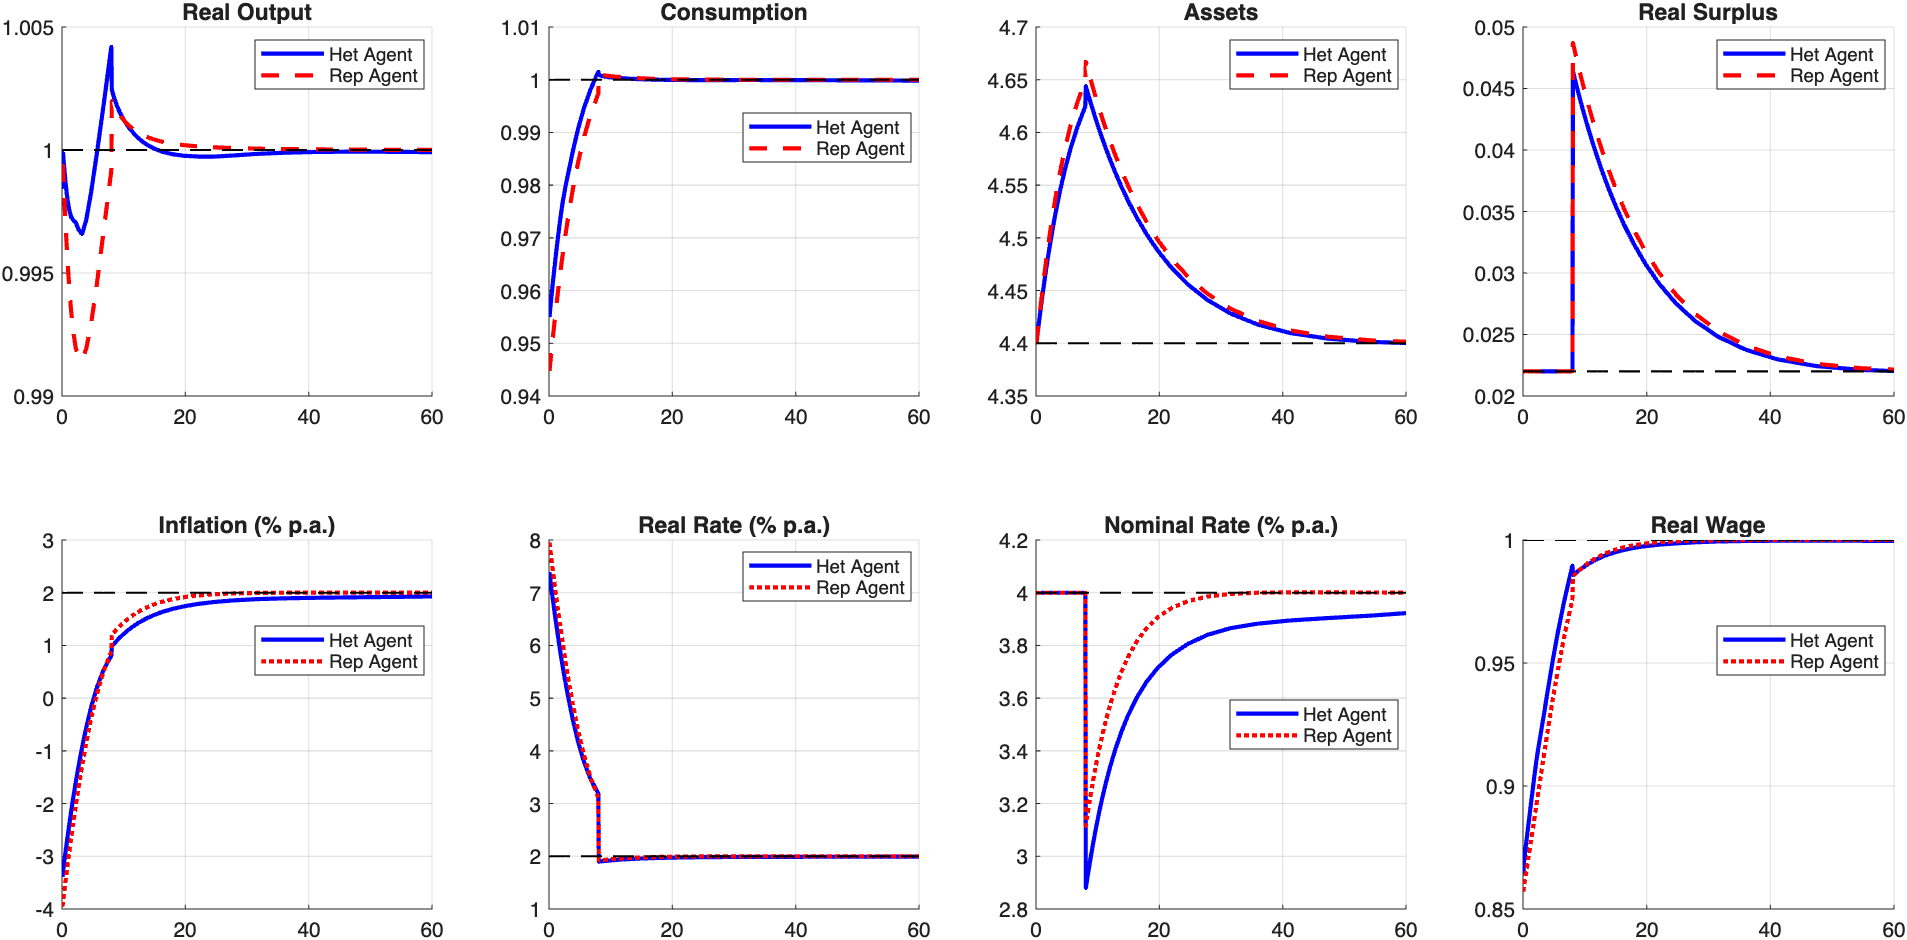
\includegraphics[width=0.8\textwidth]{Figures/TFP_known_1_HARA.png}
    \caption{Perfect foresight equilibrium after a 5\% TFP shock}
    \label{fig:tfp_known}
\end{figure}
Since agents now know that the fiscal authority will, in time, raise the primary surplus to pay down the debt accumulated initially, agents save more rapidly in the initial phase before the regime change is effected. This is enabled by a much sharper rise in the real rate, which results in agents accumulating over 5 times the assets over steady state level as opposed to the imperfect foresight equilibrium. With monetary policy pegged at the nominal rate initially, inflation sharply, inducing a deflationary phase.

A fall in marginal costs, in this case, results in a much sharper fall in real wages. With consumption falling in response to the hike in real rates, the incentive to work falls. Complemented by the large fall in real wages, effective labor supply falls sharply, offsetting the initial TFP shock altogether. Output dips below the steady state level for a short period as the TFP shock dissipates, before the rise in wages and a fall in the real rate increases the motive to consume and work, leading to an eventual increase in output above the steady state. However, the deviation in output from the steady state is less than half of the maximum deviation in the imperfect foresight equilibrium.

Once the regime change is effected, agents now consume by dissaving from the initially accumulated assets. The increase in government surplus is sharper than the previous case as the level of government debt accumulated is higher due to the higher level of asset accumulation by households. Since inflation remains below steady state level throughout, the nominal rate is cut at the point of the regime change, bringing the real rate back down close to the steady state level. Upon the regime change, all other variables smoothly return to their steady state levels. The nominal rate and inflation return to the steady state level slower in the heterogeneous agent economy than in the representative agent one.

\subsection{Discount rate shock}

\subsubsection*{Baseline: No regime change}

Again, the baseline I consider is the transition path under regime 1.
\begin{figure}[h]
    \centering
    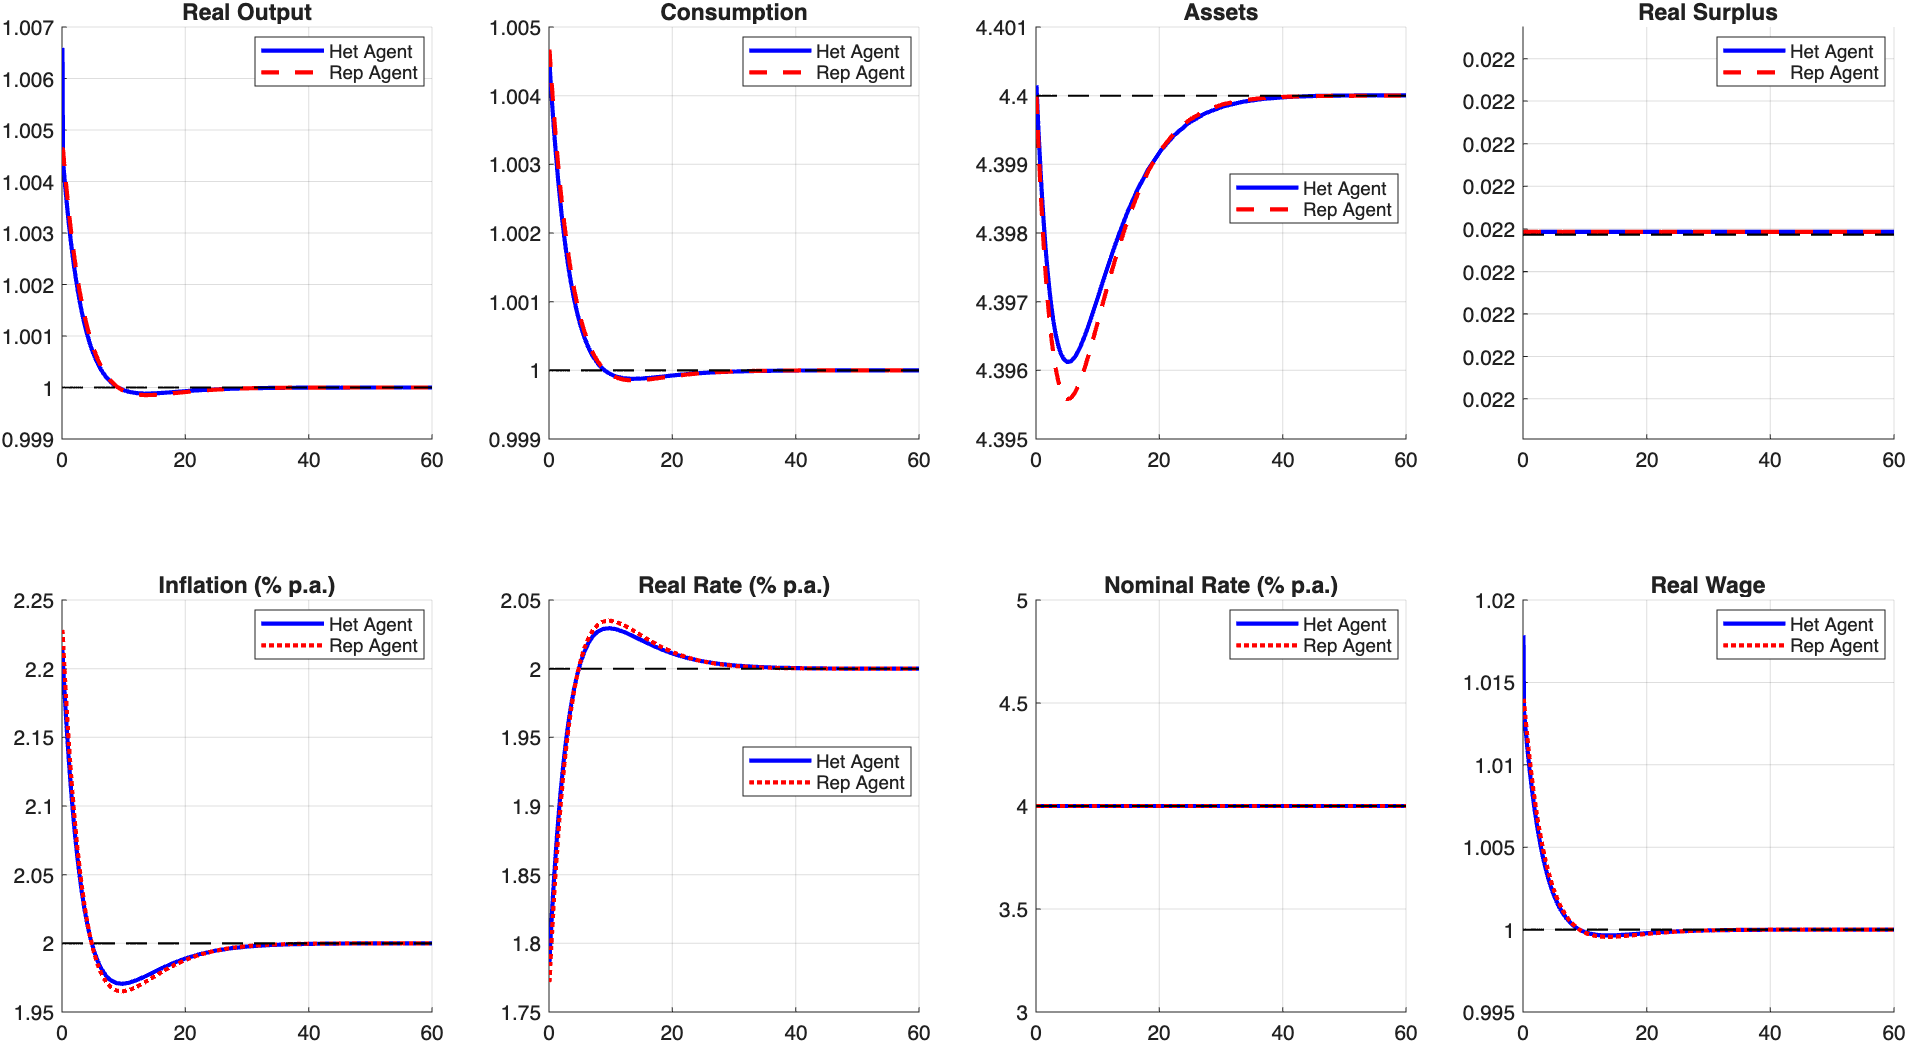
\includegraphics[width=0.8\textwidth]{Figures/disc_HARA_reg1.png}
    \caption{Transition path after a 0.001 discount rate shock: Regime 1}
    \label{fig:disc}
\end{figure}
A positive discount rate shock leads to a decrease in the intertemporal saving motive. This results in an increase in consumption and inflation, which under a pegged nominal rate and surplus, leads to a fall in the real rate. Inflation above the steady state is a result of a phase of marginal cost increases above the flexible price level, which is reflected in the real wage rising above the steady state level. While an increase in consumption decreases the incentive to work, the increase in real wages offset this, thus leading to the increase in real output.

As the shock dissipates and household assets reach a trough, consumption and inflation dip below steady state level, which leads to a rise in the real rate above the steady state level. This provides the incentive to save and a return to steady state.

\subsubsection*{Imperfect foresight equilibrium}

\begin{figure}[h]
    \centering
    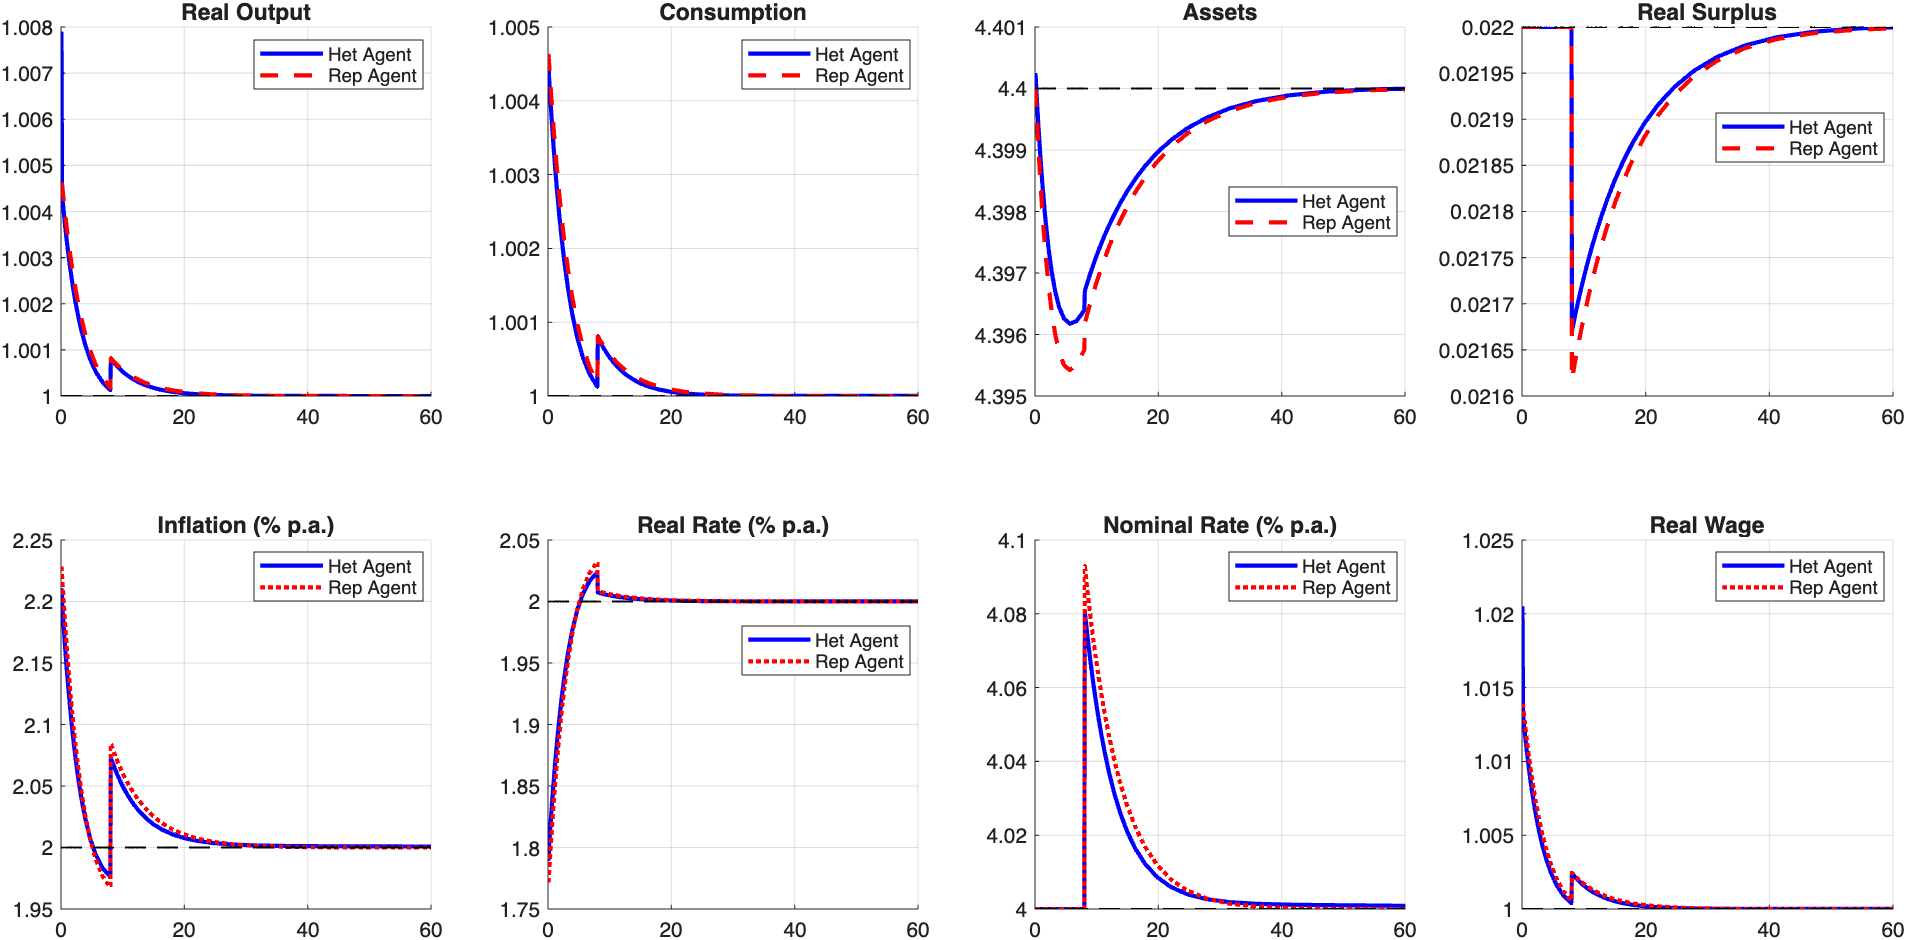
\includegraphics[width=0.8\textwidth]{Figures/disc_unknown_1_HARA.png}
    \caption{Imperfect foresight equilibrium after a 0.001 discount rate shock}
    \label{fig:disc_unknown}
\end{figure}
At the impact of the regime change, agents learn that the government will now increase the lump sum transfer above the steady state level till the economy returns to the steady state. This leads to an upward jump in consumption and decreases the incentive to work. That results in an increase in real wages and an increase in output. This creates an inflation pressure, leading to inflation jumping above the target, and a corresponding jump in the nominal rate above the steady state level. Together, these lead to a fall in the real rate closer to the steady state level, though it remains above it, providing the incentive to save and return to the steady state.

\subsubsection*{Perfect foresight equilibrium}

\begin{figure}[h]
    \centering
    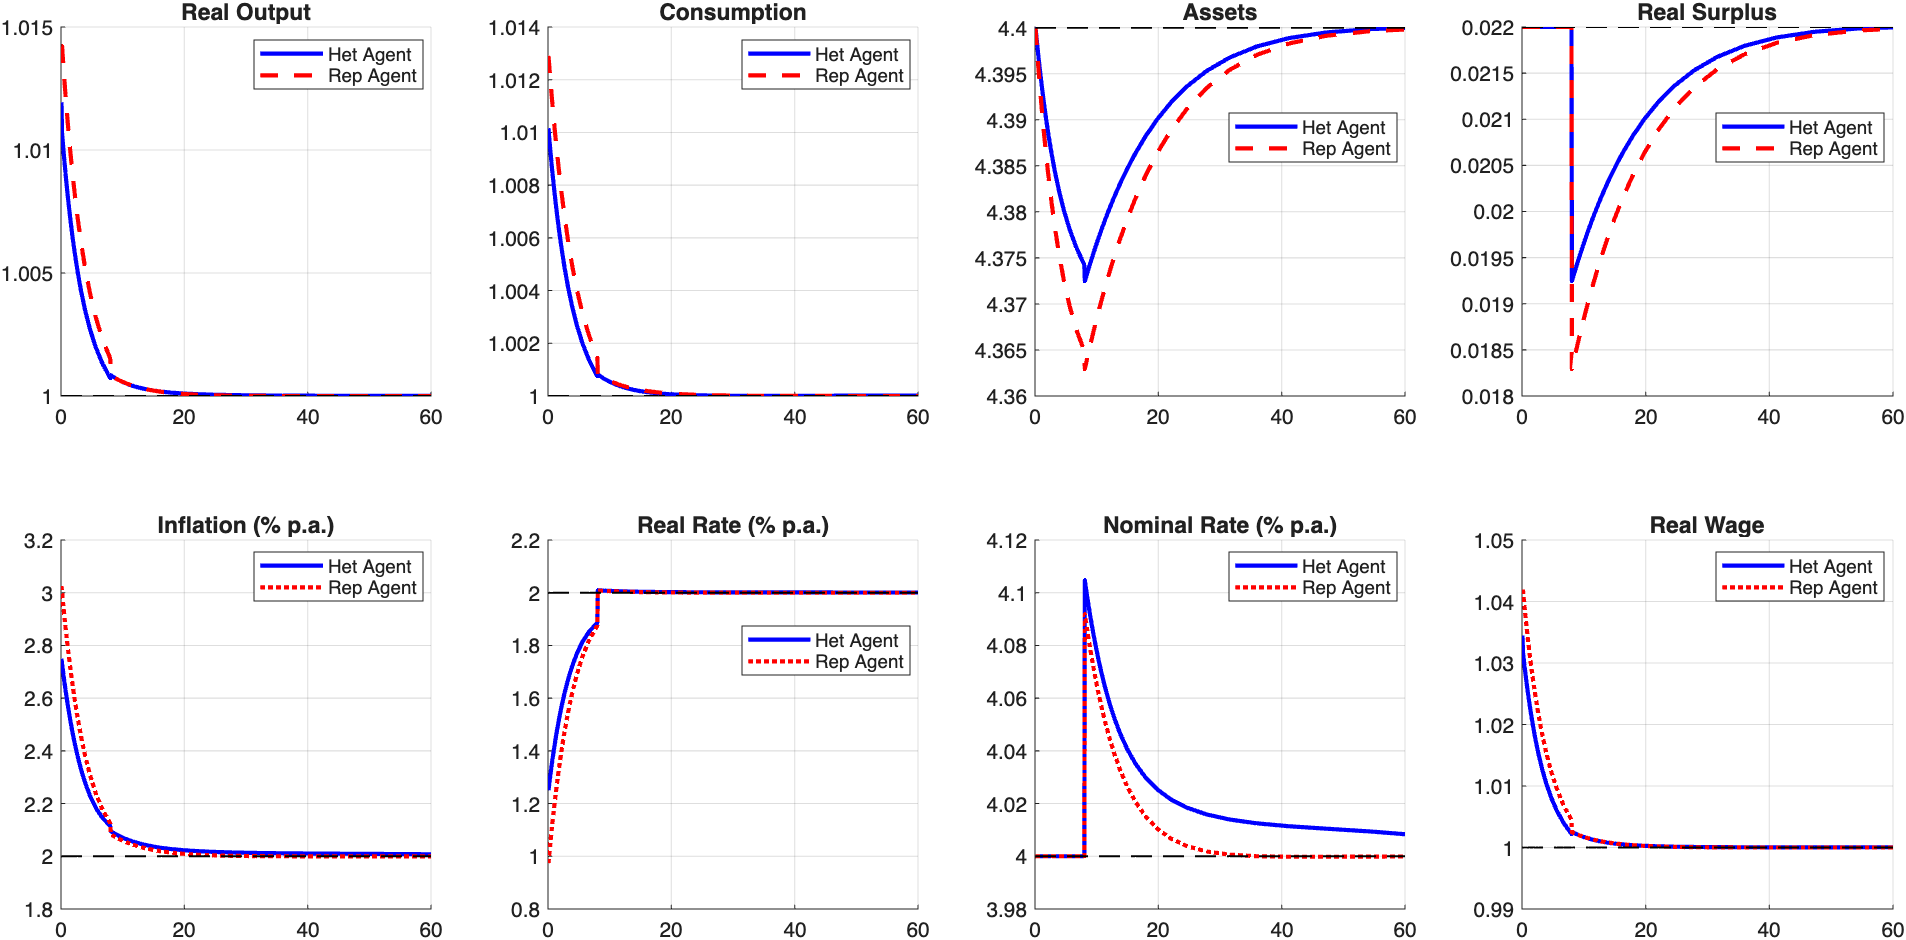
\includegraphics[width=0.8\textwidth]{Figures/disc_known_1_HARA.png}
    \caption{Perfect foresight equilibrium after a 0.001 discount rate shock}
    \label{fig:disc_known}
\end{figure}
With advance knowledge of the regime change, agents immediately increase their consumption by more than in the imperfect foresight case and dissave more, as they are aware of the increase in lump sum transfers in the future. The response of the economy, in this case, is not qualitatively very different to the case of the perfect foresight equilibrium, except for the fact that there is no overshooting of inflation and the real rate across the steady state level. The main difference between the two transition paths is quantitative.

\subsection{Discussion}

\subsubsection*{Effect of foresight about regime change}

Knowing about an impending regime change can invoke a response that might not, even qualitatively, resemble the response to the shock under either of the two regimes alone. More importantly, a regime change does not even represent a ``middle ground'' in the response between the two regimes. For instance, consider the response to the TFP shock under regime 2 alone.
\begin{figure}[h]
    \centering
    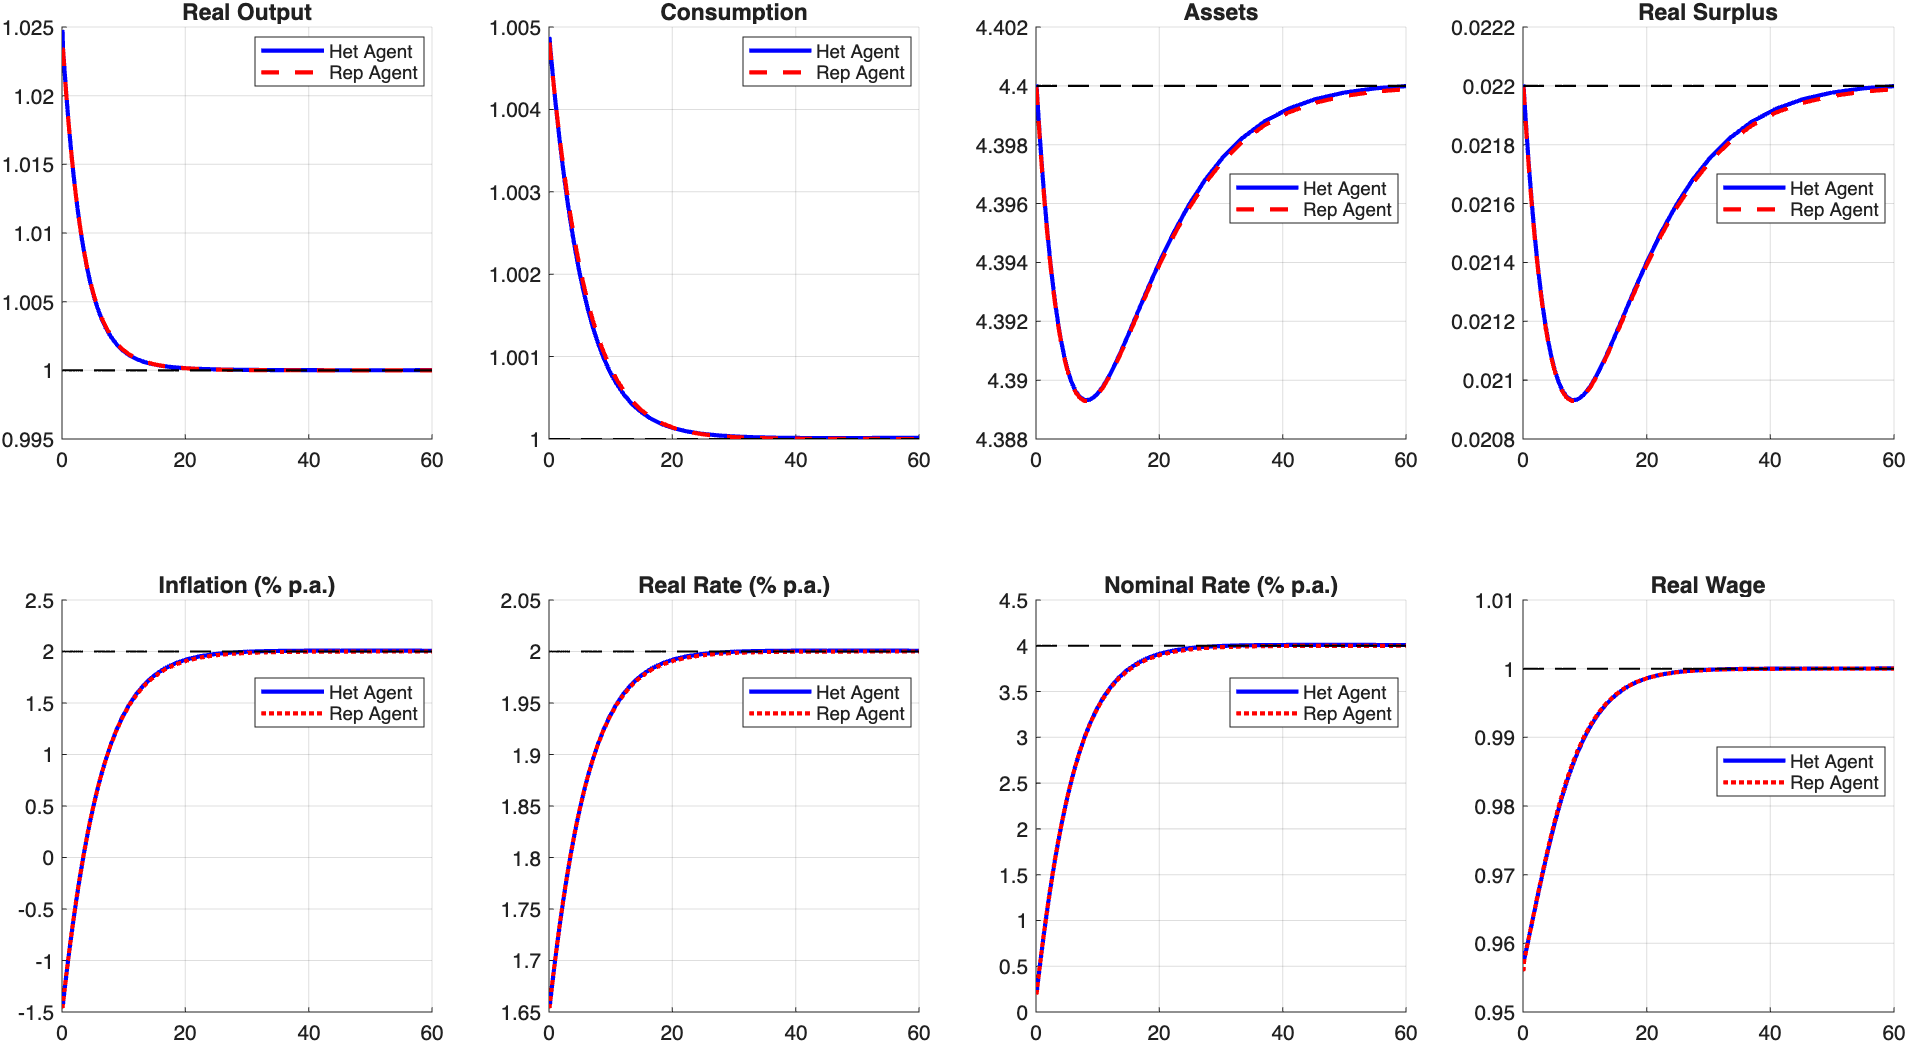
\includegraphics[width=0.8\textwidth]{Figures/TFP_HARA_reg2.png}
    \caption{Transition path after a 5\% TFP shock: Regime 2}
    \label{fig:tfp_reg2}
\end{figure}
A positive TFP shock under both regimes leads to an increase in consumption and output above the steady state. However, under the perfect foresight equilibrium, real output initially falls below the steady state level before rising above it, and consumption mostly stays below the steady state level, and only marginally exceeds it for the remainder of the transition path. Similarly, households save more under the perfect foresight equilibrium than under regime 1, even as household assets remain below steady state under regime 2.

\subsubsection*{Extension: Other regime changes and welfare effects of knowledge}

A preliminary examination of the transition paths reveal that knowing of an impending regime change might not necessarily be welfare improving. Again, the case of the TFP shock is illustrative. Unlike the imperfect foresight equilibrium, where the regime change leads to a consumption path above the steady state level throughout, the perfect foresight equilibrium leads to a consumption path that is entirely below the steady state level, even as the TFP shock is positive.

Of course, this is not definitive, given that the disutility from labor supply also features in the welfare calculation. Nevertheless, this preliminary finding suggests that the general equilibrium implications of foresight on welfare are not straightforward. Additionally, heterogeneity across households implies, just as with fiscal and monetary policy, that the welfare implications of foresight, too, might not be uniform.

Performing welfare analyses highlight how the monetary and fiscal authorities can design and communicate regime changes towards redistributing welfare across households, or perhaps even improve welfare uniformly in some cases. It might also be interesting to consider whether instituting a regime change by itself can be welfare improving, with or without advance knowledge of it.

Finally, when considering welfare effects, it would be interesting to consider a broader definition of a regime change, such as a change in the inflation target or the debt target in the fiscal rule, which can affect the subsequent steady state of the economy.

\end{document}